\documentclass[10pt]{article}
% \usepackage[letterpaper,text={6.5in,8.7in},centering]{geometry}
\usepackage{amssymb,amsmath,times,url,graphicx,amsthm,alltt}
%\usepackage[pdftex,urlcolor=blue,pdfpagemode=none,pdfstartview=FitH]{hyperref}
\usepackage{my_packages}
\usepackage{tikz_packages}
%% url smaller font.
\makeatletter
\def\url@leostyle{%
  \@ifundefined{selectfont}{\def\UrlFont{\sf}}{\def\UrlFont{\small\ttfamily}}}
\makeatother
\urlstyle{leo}

%\usepackage[all,import]{xy}

\renewcommand{\baselinestretch}{1.2}
\date{}

\renewcommand{\thesubsection}{\arabic{subsection}. }
\renewcommand{\thesubsubsection}{\arabic{subsection}.\arabic{subsubsection} }

\theoremstyle{definition}
\newtheorem{prob}{Problem}[section]
%\renewcommand{\theprob}{\arabic{section}.\arabic{prob}}
\renewcommand{\theprob}{\arabic{prob}}

\newenvironment{subprob}%
{\renewcommand{\theenumi}{\alph{enumi}}\renewcommand{\labelenumi}{(\theenumi)}\begin{enumerate}}%
{\end{enumerate}}%


\begin{document}

\pagestyle{empty}
\section*{MAE3134: Homework 3}
\vspace*{-0.4cm}
\noindent{Due date: 20 February 2018}%\\%\vspace*{0.5cm}

\begin{prob}
    A low pass filter is modeled using using the following transfer fuction:
    \begin{align}
        \bracket{s + \frac{R_1 + R_2}{R_1 R_2 C}} V_{out}(s) = \frac{1}{R_1 C} V_{in}(s) + V_{out}(0), 
    \end{align}
    where \( R_1 = \SI{40}{\kilo\ohm}, R_2 = \SI{200}{\kilo\ohm}, C = \SI{5}{\micro\farad}\).

    \begin{subprob}
        \item Find the analytical output voltage from the low pass filter assuming an input of \( V_{in}(t) = \SI{2}{\volt}\) and zero initial conditions.
        \item Use the initial and final value theorems to validate your solution.
        \item Determine the rise and settling time for this system response.
        \item Generate a plot of the response and mark on the plot the values of rise time and settling time.
    \item Your boss tells you that you actually need a different low pass filter with a rise time of \SI{0.3}{\second}.
        Your boss failed their previous linear systems class and wants to buy a new filter instead of modifying the already existing filter.
        Pick a value of \( R_2\) such that the rise time meets the specification.
    \end{subprob}
\end{prob}

\begin{prob}
    A single axis accelerometer is modeled using the following transfer function:
    \begin{align}
        \parenth{s^2 + \frac{b}{m_{pm}} + \frac{k}{m_{pm}}} X(s) = \frac{F(s)}{m_c} + s x(0) + \parenth{\dot{x}(0) + \frac{b}{m_{pm}} x(0)},
    \end{align}
    with the following parameters:
    \begin{align*}
        m_c = \SI{1}{\kilo\gram} \quad m_{pm} = \SI{0.01}{\kilo\gram} \quad b = \SI{0.2}{\newton\second\per\meter} \quad k = \SI{1}{\newton\per\meter}
    \end{align*}

    \begin{subprob}
        \item Find the analytical output response \( x(t) \) if \( f(t) = \SI{30}{\newton}\) and the initial conditions are zero.
        \item How does the response change if \( x(0) = \SI{0.1}{\meter} \) and \( \dot{x}(0) = 0 \)?
        \item Use the initial and final value theorems to validate your solutions to the previous questions.
        \item You discover that you'd like a different response so you naively modify the system parameters:
            \begin{align*}
        m_c = \SI{1}{\kilo\gram} \quad m_{pm} = \SI{0.01}{\kilo\gram} \quad b = \SI{0.02}{\newton\second\per\meter} \quad k = \SI{0.1}{\newton\per\meter}.
            \end{align*}
            What is the analytical output response if \( f(t) = \SI{30}{\newton} \) and zero initial conditions?
            Find the rise time, settling time, peak time, and percent overshoot for this response.
        \item Generate a plot with all three output responses.
        \item Discuss the differences between the responses from part A and part D.
            Which response is more acceptable for an accelerometer?
    \end{subprob}
\end{prob}
  
\clearpage\newpage
\begin{prob}
    You're trying to ``tune'' a high pass filter,  by simply guessing no less!
    The filter is defined by
    \begin{align}
    \bracket{s + \frac{R_1 + R_2}{R_1 R_2 C} } V_{out}(s) = s V_{in}(s) + V_{out}(0) ,
    \end{align}
    where \( R_1 = \SI{40}{\kilo\ohm}, R_2 = \SI{200}{\kilo\ohm}, C = \SI{5}{\micro\farad}\).
    \begin{subprob}
    \item Find the analytical output response for \( v_{in}(t) = 10 \sin 0.6 t \) with zero initial conditions.
    \item Find the analytical output response for \( v_{in}(t) = 10 \sin 60 t \) with zero initial conditions.
    \item  Generate a plot with both responses and discuss how effective this design is for a \textbf{HIGH} pass filter.
    \end{subprob}
\end{prob}


\begin{prob}
    \begin{figure}[h]
        \centering
        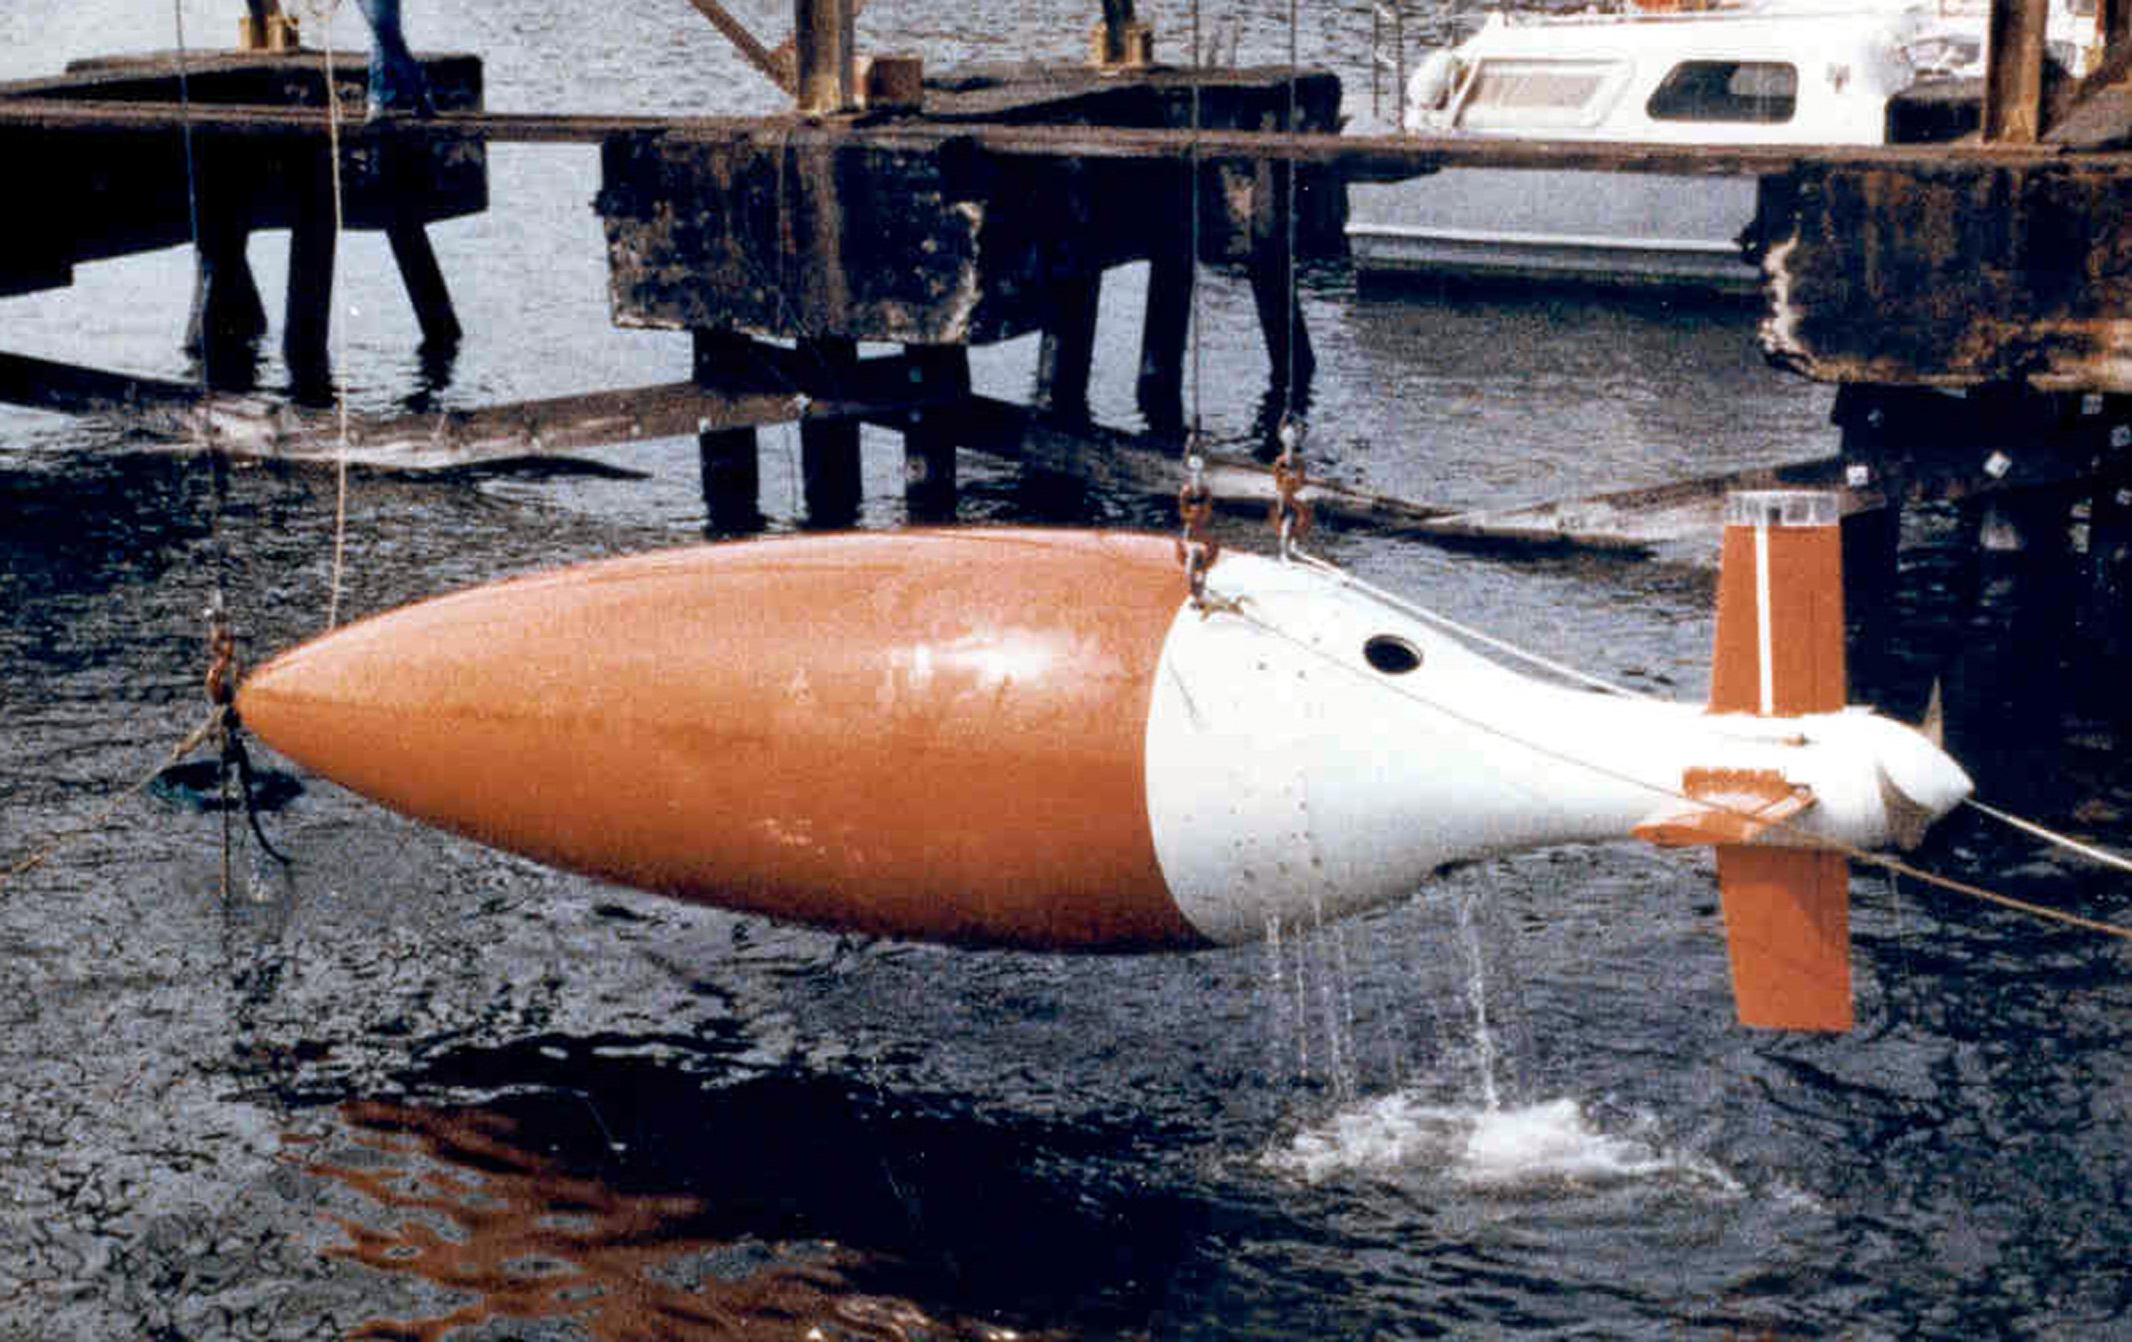
\includegraphics[width=0.5\textwidth]{figures/UFSS-TEST-PHOTO-1.jpg}
        \caption{Submersible Vehicle~\label{fig:vehicle}}
    \end{figure}
    The transfer function relating the pitch angle, \( \theta (s) \), to the elevator deflection angle, \( \delta e (s) \), for an Unmanned Free-Swimming Submersible, shown in~\cref{fig:vehicle}, is given by
    \begin{align}
        \frac{\theta (s) }{\delta e(s)} = \frac{-0.125 (s + 0.435)}{(s+1.23)(s^2 + 0.226 s + 0.0169)} .
    \end{align}

    \begin{subprob}
    \item Using only the second order poles from the transfer function predict the percent overshoot, rise time, peak time and settling time.
    \item Using the Laplace transform, find the analytical expression for the pitch angle response to a step input of the elevator.
    \item Evaluate the effect of the additional pole and zero on the validity of the second order approximation.
    \item Plot the step response of the vehicle dynamics and verify your conclusions on the effect of the additional pole and zero.
    \end{subprob}
\end{prob}

\clearpage\newpage
\begin{prob}
    \begin{figure}[h]
        \centering
        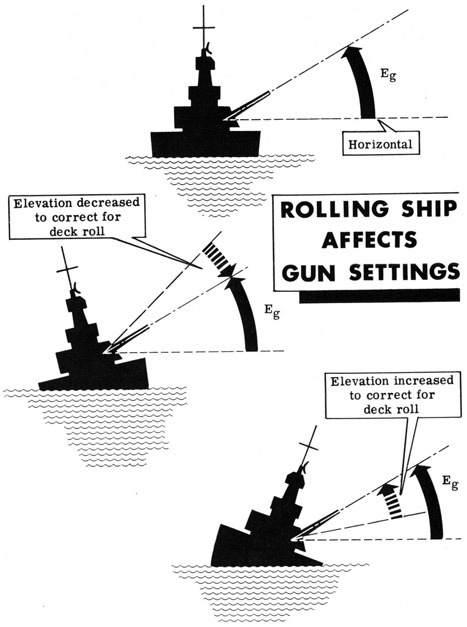
\includegraphics[width=0.5\textwidth]{figures/partd-03.jpg}
        \caption{Rolling Ship on Gun accuracy~\label{fig:gun}}
    \end{figure}
    Ships at sea undergo motion about their roll axis, as demonstrated in~\cref{fig:gun}.
    Fins called stabilizers are used to reduce this rolling motion.
    The stabilizers can be positioned by a closed-loop roll control system that consists of actuator, such as fins or thrusters, and sensors, such as gyroscopes or accelerometers, as well as a model of the ship dynamics.
    Assume the roll dynamics, which relates the roll angle output, \( \theta (s) \) to a disturbance torque input, \( T_D(s)\), is given by
    \begin{align}
        \frac{\theta(s)}{\T_D(s)} = \frac{2.25}{s^2 + 0.5 s + 2.25} .
    \end{align}

    Accomplish the following:
    \begin{subprob}
        \item Find the natural frequency, damping ratio, peak time, settling time, rise time, and percent overshoot.
        \item Find the analytical expression for the output response to a unit step input.
        \item Use a computer tool to verify your solutions and plot the response to a step input.
        \item Plot the location of the poles on the complex plane. 
            In addition, mark the values of damping ratio and natural frequency on your plot.
        \item Do you believe this roll response is acceptable for a ship in response to an input disturbance?
    \end{subprob}
\end{prob}
\end{document}

